\subsection{POSIX}
POSIX (\acrlong{posix}) ist eine Erweiterung zum IEEE 1003, welche die API, Shell und Utilities von UNIX standartisierte.
Ursache für POSIX war, dass UNIX Software nicht auf allen UNIX Systemen lief.
Durch diese Standardisierung soll ein Skript oder Programm portierbar sein, ohne das eine Änderung im Sourcecode vorgenommen werden muss. Der Vorteil liegt darin, dass es auf jedem System läuft. Dadurch wird jedoch der technische Fortschritt stark abgebremst, weil es auch auf dem ältesten System laufen soll, welches z.B. ein 8 Bit Prozessor besitzt. Wenn man z.B. die Shell betrachtet, muss alles für \textit{sh}, der originalen Bourne Shell, kompatibel sein. \cite{shotts2012linux}



\begin{figure}[ht]
  \begin{center}
  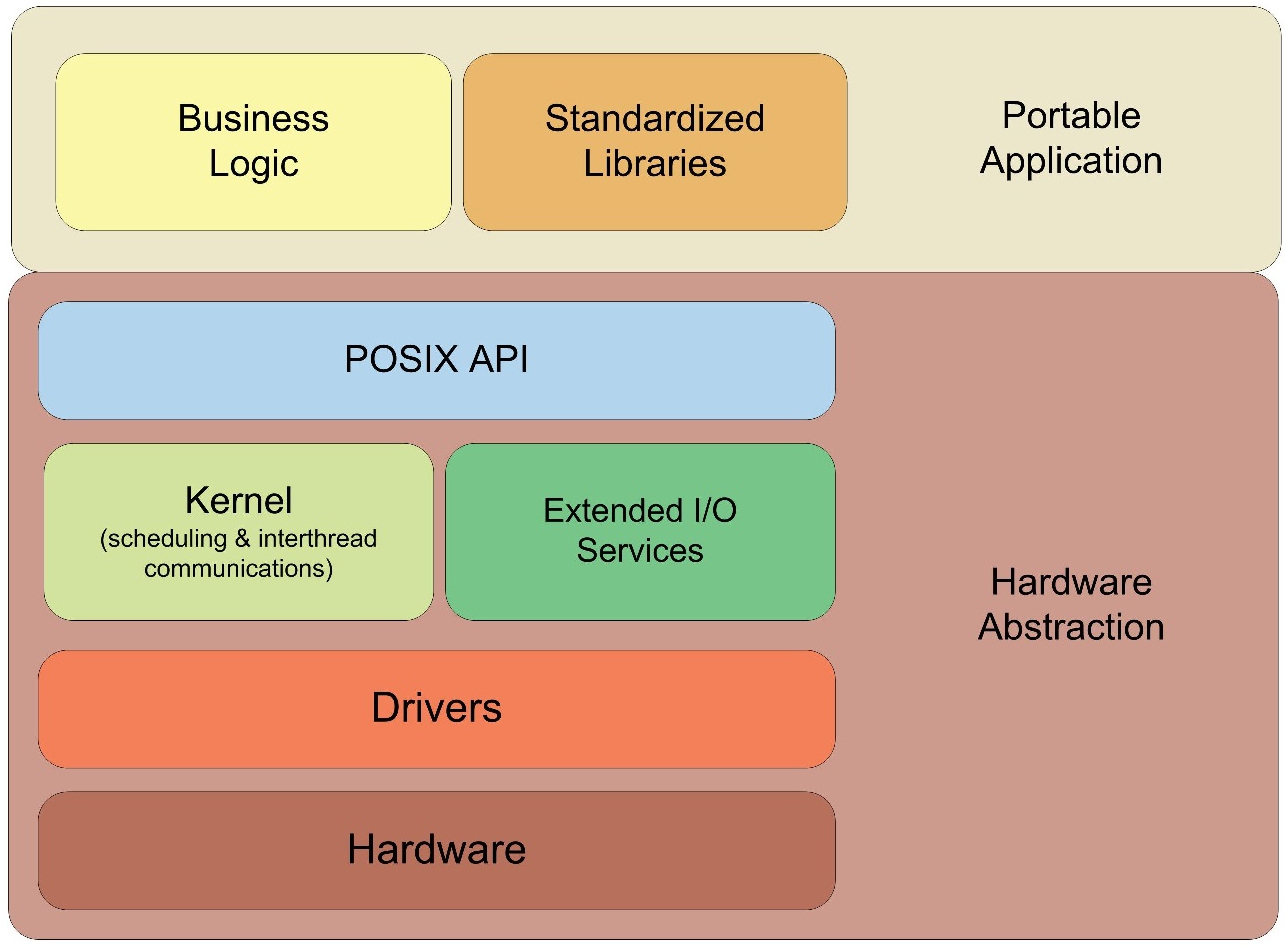
\includegraphics[width=0.48\textwidth]{pic/20_pixhawk/POSIX_RTOS_Model.jpg}
  \caption{POSIX API}
  \cite{posix_pic}
  \label{fig:posix}
  \end{center}
\end{figure}


\noindent In der Abbildung \ref{fig:posix} ist ersichtlich, wie die Applikation durch den POSIX Layer von der Hardware getrennt wird. Dieses POSIX API stellt einfache Interfaces zur Verfügung, welche im Kernel oder dem erweiterten I/O Service implementiert wurden. \\
Die Applikation kann nun auf jede Hardware portiert werden, da sie klar definierte Funktionen verwendet.

\clearpage